\documentclass[12pt,a4paper]{article}

\usepackage[cm]{fullpage}
\usepackage{amsthm}
\usepackage{amsmath}
\usepackage{amsfonts}
\usepackage{amssymb}
\usepackage{xspace}
\usepackage[english]{babel} % Used for date formatting
\usepackage{fancyhdr}
\usepackage{titling}
\usepackage{url}
\usepackage{csquotes}
\usepackage[
    style=numeric,
    bibstyle = numeric,
    citestyle = numeric,
    sorting = none,
    backend=biber
]{biblatex}
\usepackage{parskip}
\usepackage{graphicx}
\usepackage{subcaption}
\usepackage{hyperref}
\usepackage{listings}
\usepackage[table,xcdraw]{xcolor}
\usepackage{nameref}
\graphicspath{ {./img/} }
\addbibresource{summary.bib}

\usepackage{multirow}
\usepackage{listings}
\usepackage[yyyymmdd]{datetime}

\usepackage{mdframed}
\usepackage{lipsum}

\newmdtheoremenv{theo}{Theorem}

%%%%%%%%%%%%%%%%%%%%%%%%%%%%%%%%%%%%%%%%%
% - Declare some maths operators
%%%%%%%%%%%%%%%%%%%%%%%%%%%%%%%%%%%%%%%%%
\DeclareMathOperator*{\argmax}{argmax}

%%%%%%%%%%%%%%%%%%%%%%%%%%%%%%%%%%%%%%%%%
% - Declare langle and rangle in text
%%%%%%%%%%%%%%%%%%%%%%%%%%%%%%%%%%%%%%%%%
\newcommand{\<}[1]{\guilsinglleft}
\renewcommand{\>}[1]{\guilsinglright}

%%%%%%%%%%%%%%%%%%%%%%%%%%%%%%%%%%%%%%%%%
% - Format date to ''dd.mm.YYYY''
%%%%%%%%%%%%%%%%%%%%%%%%%%%%%%%%%%%%%%%%%
\DefineBibliographyExtras{english}{%
  \protected\def\mkbibdateshort#1#2#3{%
    \iffieldundef{#3}
      {}
      {\mkdayzeros{\thefield{#3}}%
       \iffieldundef{#2}{}{.}}%
    \iffieldundef{#2}
      {}
      {\mkmonthzeros{\thefield{#2}}%
       \iffieldundef{#1}{}{.}}%
    \iffieldbibstring{#1}
      {\bibstring{\thefield{#1}}}
      {\dateeraprintpre{#1}\mkyearzeros{\thefield{#1}}}}%
  \protected\def\mkbibdatelong#1#2#3{%
    \iffieldundef{#3}
      {}
      {\stripzeros{\thefield{#3}}%
       \iffieldundef{#2}{}{\nobreakspace}}%
    \iffieldundef{#2}
      {}
      {\mkbibmonth{\thefield{#2}}%
       \iffieldundef{#1}{}{\space}}%
    \iffieldbibstring{#1}{\bibstring{\thefield{#1}}}{\stripzeros{\thefield{#1}}}}%
}


% - Format other dates to ''YYYY-mm-dd''
\renewcommand{\dateseparator}{-}


%%%%%%%%%%%%%%%%%%%%%%%%%%%%%%%%%%%%%%%%%
% - Define LST-LISTINGS
%%%%%%%%%%%%%%%%%%%%%%%%%%%%%%%%%%%%%%%%%
\definecolor{backcolor}{rgb}{0.95,0.95,0.92}

\lstdefinestyle{mystyle}{
    backgroundcolor=\color{backcolor},
    breaklines=true,
    numbers=left,
    numbersep=5pt,
    basicstyle=\ttfamily\footnotesize,
    captionpos=b
}

\lstset{style=mystyle}

%%%%%%%%%%%%%%%%%%%%%%%%%%%%%%%%%%%%%%%%%%
% This part needs customization from you %
%%%%%%%%%%%%%%%%%%%%%%%%%%%%%%%%%%%%%%%%%%

% your group number your names and matriculation numbers here
\newcommand{\groupnumber}{1}
\newcommand{\name}{Alexander Beiser}
\newcommand{\matriculation}{To: The masses}
\newcommand{\gt}{\ensuremath >} 

%%%%%%%%%%%%%%%%%%%%%%%%%%%%%%%%%%%%%%%%%%
%           End of customization         %
%%%%%%%%%%%%%%%%%%%%%%%%%%%%%%%%%%%%%%%%%%

\newcommand{\projnumber}{1}
\newcommand{\Title}{Summary}
\setlength{\headheight}{15.2pt}
\setlength{\headsep}{20pt}
\setlength{\textheight}{680pt}
\pagestyle{fancy}
\fancyhf{} 
\fancyhead[L]{Clinguin - Project Document}
\fancyhead[C]{}
\fancyhead[R]{\name}
\renewcommand{\headrulewidth}{0.4pt}
\fancyfoot[C]{\thepage}


\begin{document}
\thispagestyle{empty}
\noindent\framebox[\linewidth]{%
 \begin{minipage}{\linewidth}%
 \hspace*{5pt} \textbf{Clinguin (Summer 2022)} \hfill University of Potsdam - Potassco
 \hspace*{5pt}\\

 \begin{center}
  {\bf\Large Clinguin Project Document}
 \end{center}

 \vspace*{5pt}\hspace*{5pt} \today\hfill Clinguin\hspace*{5pt}
\end{minipage}%
}
\vspace{0.5cm}
%%%%%%%%%%%%%%%%%%%%%%%%%%%%%%%%%%%%%%%%%%%%%%%


%\begin{center}
%\textbf{\name} %please fill the information above

%\matriculation %please fill the information above
%\end{center}
%%%%%%%%%%%%%%%%%%%%%%%%%%%%%%%%%%%%%%%%%%%%%%%


\section{Ideas}


%%%%%%%%%%%%%%%%%%%%%%%%%%%%%%%%%%%%%%%%%
% Timestamp: 04.-11.07.2022
%%%%%%%%%%%%%%%%%%%%%%%%%%%%%%%%%%%%%%%%%
\subsection{Project Summary}

\noindent The \textit{Clinguin} project can be seen as a language extension to a Logic-Program, which adds the functionality to create a User-Interface (UI). Capability wise the UI shall be capable of dynamic updates, i.e. not just a static display of a stable-model(s), but a program where one can interact with the logic program.\\
An example for this is the Sudoku problem. Using the Clinguin one is able to generate a Sudoku playing-field, where the field is interactive in a sense, that if one selects one of the possible values a single field may have, the program automatically updates the not selected values and fills them in, if only one possibility exists. This is similar to forward checking for Constraint-Satisfactory-Problems (CSPs).\\

\subsection{Prototype}

\noindent Susana Hahn has written a prototype, which implements the Sudoku example from above. The used programming language is Python, further Clingo libraries (like the Clingo-Object-Relational-Mapper (CLORM)) are and the UI-framework tkinter (https://docs.python.org/3/library/tkinter.html) are used. Syntactically the prototype provides an extension by the following keywords (predicates which are used as keywords/tokens):

\begin{itemize}
    \item \textit{window(\< aattribute-name\> ,,\< aargument-key\>,,\<aargument-value\>))} - Defines the general structure/size/etc. of the displayed field
    \item \textit{widget(\< ttype-name\>,,\<uui-id\>,,\<mmaster-id\>))} - Adds a widget (ui-element/item) to the view. The accepted types are \textit{frame} (container) and \textit{menu} (dropdown menu). The \textit{ui-id} should be unique and the \textit{master-id} represents the enclosing item (for top-level frames this is the \textit{window}).
    \item \textit{geo(\<uui-id\>,,\<uui-layout\>,,\<aargument-key\>,,\<aargument-value\>))} - Used for specifying the exact location of a widget. The \textit{ui-id} is of a widget, the \textit{ui-layout} can be chosen from a tuple of \textit{(grid, place, pack)}, the \textit{argument-key} is used for specifying what one wants to set (e.g. row) and the \textit{argument-value} is the corresponding value.
    \item \textit{config(\<uui-id\>,,\<aargument-key\>,,\<aargument-value\>))} - The \textit{ui-id} is of the corresponding widget, the \textit{argument-key} is the property to set (e.g. font width or some color) and the \textit{argument-value} is the corresponding value to the key.
    \item \textit{opt(\<uui-id\>,,\<vvalue\>,,\<ooriginal-state\>))} - This is used for the dynamic updates of the gui. The \textit{ui-id} is for the corresponding widget. In the prototype the stable matches are computed via the \textit{brave} option, and for each possible value the \textit{original-state} can have, also one \textit{opt} is generated. This is used for computing what values a single sudoku field may have.
\end{itemize}

\noindent In general the program works like this: The program scans the logic-program for the syntactic elements above, and then creates the ui with the elements (function \textit{create\_layout()}, uses cautious reasoning). Then the dropdown-menus (i.e. the Sudoku cells) are filled, with the function \textit{update\_options()} (uses brave reasoning). Here for each such dropdown-menu a callback function is added, which when clicked adds an assumption, that a certain value must be used for the sudoku field. Then the process repeats itself.

\subsection{Architecture Proposals}


\subsubsection{Initial Thoughts}

\noindent The architecture of Clinguin should be flexible in a sense, that it should be compatible with several UI-Libraries/-frameworks. Further it should be efficient (which is not handled at this point, but e.g. incremental updates can be made instead of full updates).\\
The need for flexibility leads to the conclusion, that the program may not directly construct the \textit{tkinter} (or some other frameworks) window, but must create an internal representation first (See Figure \ref{fig:arch-overview}):


\begin{figure}[ht]
    \begin{center}
    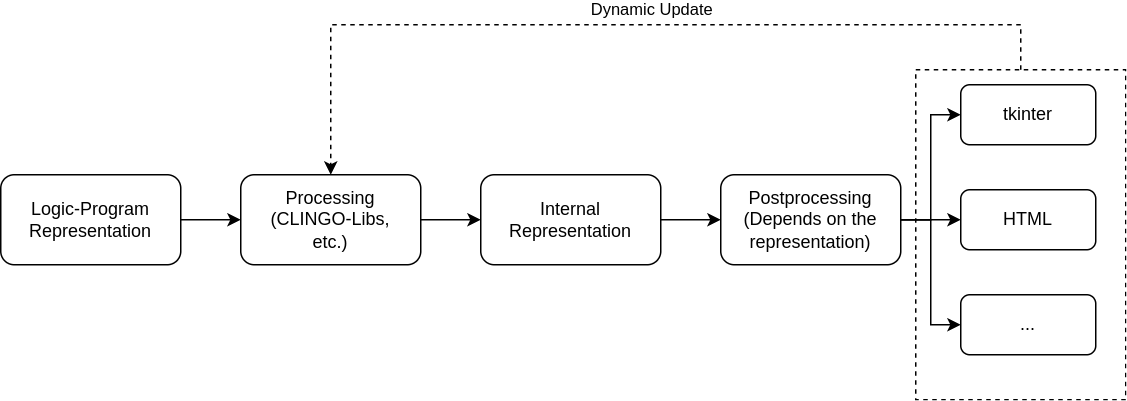
\includegraphics[width=0.7\textwidth]{imgs/overview.png}
    \caption{Informal idea of the workings of the program}
    \label{fig:arch-overview}
    \end{center}
\end{figure}

\noindent Therefore for the construction of the program a few things have to be defined/thought about:
 
\begin{enumerate}
    \item Logic-Program Representation
    \begin{itemize}
        \item Syntax of language extension
        \item Initial starting point \(\rightarrow\) syntax of prototype
        \item In general the syntax should be defined in a way that helps understanding of the program
    \end{itemize}
    \item Processing 
    \begin{itemize}
        \item Produces internal representation from the logic program
        \item Main thing: Efficiency
        \item Other things: Libraries to use (depends on selected internal representation), etc.
    \end{itemize}
    \item Internal Representation
    \begin{itemize}
        \item \textbf{Very important to think about now}: Many different options exist, like \textit{XML}, \textit{Json}, \textit{Class-Hierarchy}, \textit{HTML}, ...
        \item Different representations have different pros/cons:
        \begin{itemize}
            \item XML - Pro: Clearly defined structure, portable format. Cons: Format needs to be parsed again before it can be used (efficieny loss), postprocessing will be pretty complex
            \item Json - Pro: For hierarchical GUI tools postprocessing will not be that much, portable format. Cons: Format needs to be parsed again, for non hierarchical GUI tools postprocessing will be quite complex
            \item Class-Hierarchy - Pro: Efficiency, for hierarchical GUI tools postprocessing will be relatively easy. Cons: Non portable format (one is limited to Python represetation), for non hierarchical GUI tools postprocessing will be quite complex.
            \item HTML - Pro: Direct representation of GUI elements, i.e. one can directly view the html, otherwise similar to XML. Cons: For other views than HTML postprocessing will be pretty complex
        \end{itemize}
    \end{itemize}
    \item Postprocessing
    \begin{itemize}
        \item Depends entirely on the chosen internal representation and chosen GUI-framework
        \item Could be implemented as a \textit{1:1} match between internal representation and GUI-framework, which would lead to a modularization of the Clinguin
        \item Efficiency will be important here...
    \end{itemize}
    \item Initial GUI-Framework to use (tkinter, web/HTML, other)
\end{enumerate}


\subsubsection{Monolithic Custom}

\noindent \textbf{Hard-Coded-Monolith}: The idea is to think of an architecture, which is a monolith. The architecture should be designed in a way that fulfills most requirements. One requirement which would be hard to fulfill is the Json/Independability requirement, i.e. that the gui may be switched in the future.\\[1em]
\noindent \textbf{Json-Monolith}: It is also possible to implement it with Json as intermediary representation, to achive a seperation between gui and the rest. This approach is essentially the same as the Client-Server approach (be sure to look at it first in Section \ref{subsubsec:client-server}), just that for the message passing no server is needed, but is instead done via function calls or events. With this approach one needs to implement a lot from the Client-Server part, just without setting up a server. The downside of this approach is, that one can only use gui-frameworks from the selected programming language (i.e. Python).\\[1em]
I didn't explore on these ideas much further, but it should definitely be possible, if one drops the independability/modularization.

\subsubsection{Monolithic Model-View-Controller (MVC)}

\noindent As the MVC pattern is a widely spread Gui-Architectural pattern it makes sense to consider it. In Figure \ref{fig:mvc} the general idea of MVC is depicted, where normally there exists one such MVC-triad per GUI element, e.g. one for the top level gui element, which contains ''children'', like menu-bar, grid-controller, etc. (as depicted in Figure \ref{fig:mvc-hierarchy}).\\


\begin{figure}[ht]
    \begin{center}
    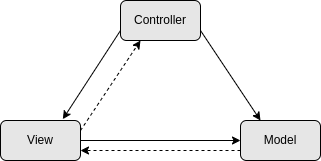
\includegraphics[width=0.4\textwidth]{imgs/mvc.png}
    \caption{General MVC idea}
    \label{fig:mvc}
    \end{center}
\end{figure}

\begin{figure}[ht]
    \begin{center}
    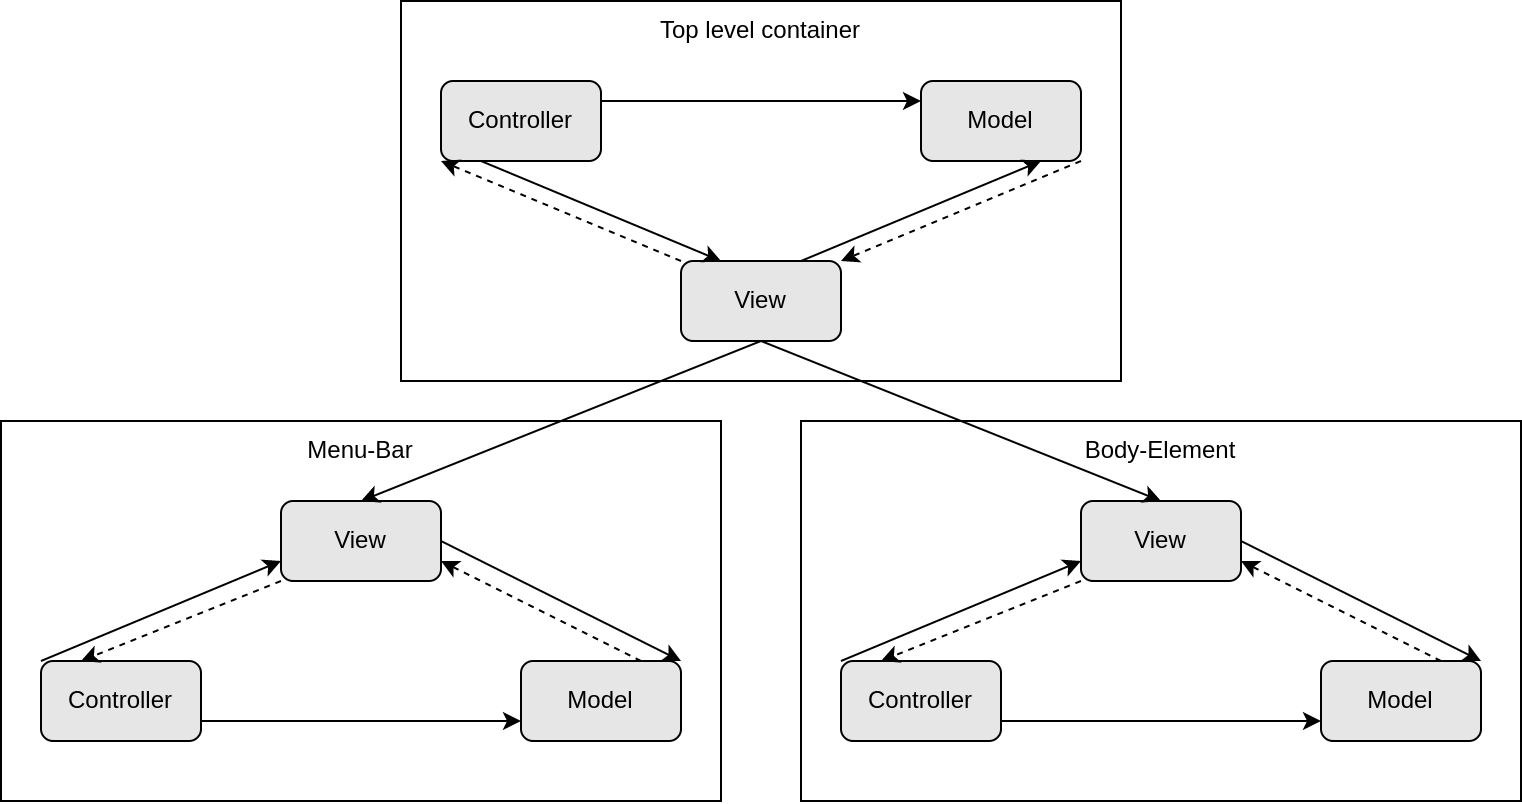
\includegraphics[width=0.7\textwidth]{imgs/mvc-architecture.png}
    \caption{MVC Hierarchy}
    \label{fig:mvc-hierarchy}
    \end{center}
\end{figure}

\noindent For Clinguin this architecture open two possible tracks of implementation, where it seems to be the case that for both tracks it would be pretty hard to get the callbacks right while using an independent representation like Json.\\[1em]
My main reason of concern in both cases is how would the notification process (callbacks) work together with Json?\\
As far as I know, when using MVC one ''hard-codes'' the View, the Controller and the Model, each in a seperate file, where then a framework (like Windows-Presentation-Foundation (WPF) for C\# - which is actually the MVVM principle, but pretty similar...) connects the files.\\
On the other hand, when one uses Json as a means for the intermediate representation, one normally uses some kind of Message-Oriented-Architecture (MOA), like a simple Client-Server system.\\

\begin{itemize}
    \item Implementation of Clinguin as a single MVC triad
    \begin{itemize}
        \item Implementing this in a way, that multiple elements are handled in one MVC should violate the MVC design principle
        \item Normally in MVC the View should be static in a sense, that the elements of a view doesn't change, just the content - but here this would be violated
        \item When using Json for data transfer, I can't imagine how the callbacks should work
    \end{itemize}
    \item Implementation of Clinguin as a MVC hierarchy
    \begin{itemize}
        \item Either as a code generator (i.e. a program which generates the python code, should fulfill the MVC design principle, but seems to be hard to implement)
        \item Or implement it just via OOP - but which would still be hard and it would even be harder to get the callbacks right.
        \item When using Json for data transfer, I can't imagine how the callbacks should work
    \end{itemize}
\end{itemize}


\subsubsection{Version 0: Simple Message based approach (Client-Server)}
\label{subsubsec:client-server}

\noindent The next option to look at is the Client-Server approach. The main point for this architecture is the flexibility, that one can use the Json data as an intermediate representation and use whatever gui one finds suitable. Further the architecture is straightforward (also the callbacks).\\
The server architecture could be implemented as a normal layered-architecture, where the data layer is responsible for the communication with the underlying logical-data-structrure (i.e. CLORM), the logic layer contains some business logic (might actually not be necessary) and the presentation layer handles incoming requests, processes them (i.e. forwarding to the logic/data-layers) and then formats the response as a Json.\\[1em]
The Client just gets the Json and constructs with this information a gui. If a user clicks on a field a request is sent to the server, which processes it, computes the stable models, etc. . Implementation wise the client can be constructed in a variety of different ways, a straightforward one would be that the Json contains enough information that one may construct a gui with possible actions and if an action occurs, sends it back. The client may be written in any programming language. \\[1em]
Another pro: When one uses a \textit{REST}-API, then 
One drawback with this approach is, that the development time might be higher than with a monolithic approach, but definitely still acceptable.

\begin{figure}[ht]
    \begin{center}
    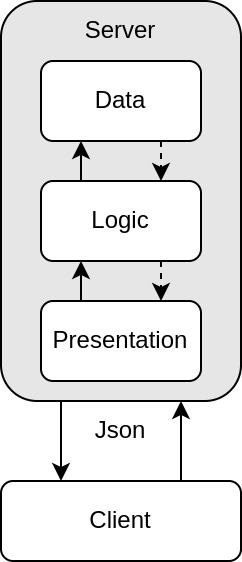
\includegraphics[width=0.2\textwidth]{imgs/client-server.png}
    \caption{Cient-Server approach}
    \label{fig:client-server-v0}
    \end{center}
\end{figure}

\noindent One could use the following libraries for this:

\begin{itemize}
    \item Server
        \begin{itemize}
            \item FastAPI - A REST framework which is similar to JavaSpringBoot or NestJS, released in 2018, high performance and seems to be maintained regularly
            \item Flask - The standard tool for developing REST Api's in Python (syntactically similar to NestJS and Java Spring Boot). Seems to be not that great in terms of performance
        \end{itemize}
    \item Client
        \begin{itemize}
            \item api-client - seems to be exactly what we need 
        \end{itemize}
\end{itemize}

\noindent Further one can package both together, that from the outside it seems like, it is just one program, although they are two in fact. In terms of endpoints/APIs only three are proposed:

\begin{itemize}
    \item GET: ''/health'' - For startup process, check if server is running
    \item GET: ''/'' - Get Json data to display
    \item POST: ''/'' - Send server, what has been clicked, etc.
\end{itemize}

\newpage
\subsubsection{Version 1: Simple Message based approach (Client-Server)}

\noindent Based on the \textit{Version 0} of the simple message based approach, the new approach (besides the flexibility granted by the intermediate Json format) addresses two other important tasks:

\begin{itemize}
    \item Making the server-solver as flexible as possible, that it can be switched out/in.
    \item A concept structure of a \textit{tkinter} frontend.
\end{itemize}

\noindent The figure \ref{fig:client-server-v1} displays the advanced architecture on a high level, so one gets an idea how this works:

\begin{figure}[ht]
    \begin{center}
    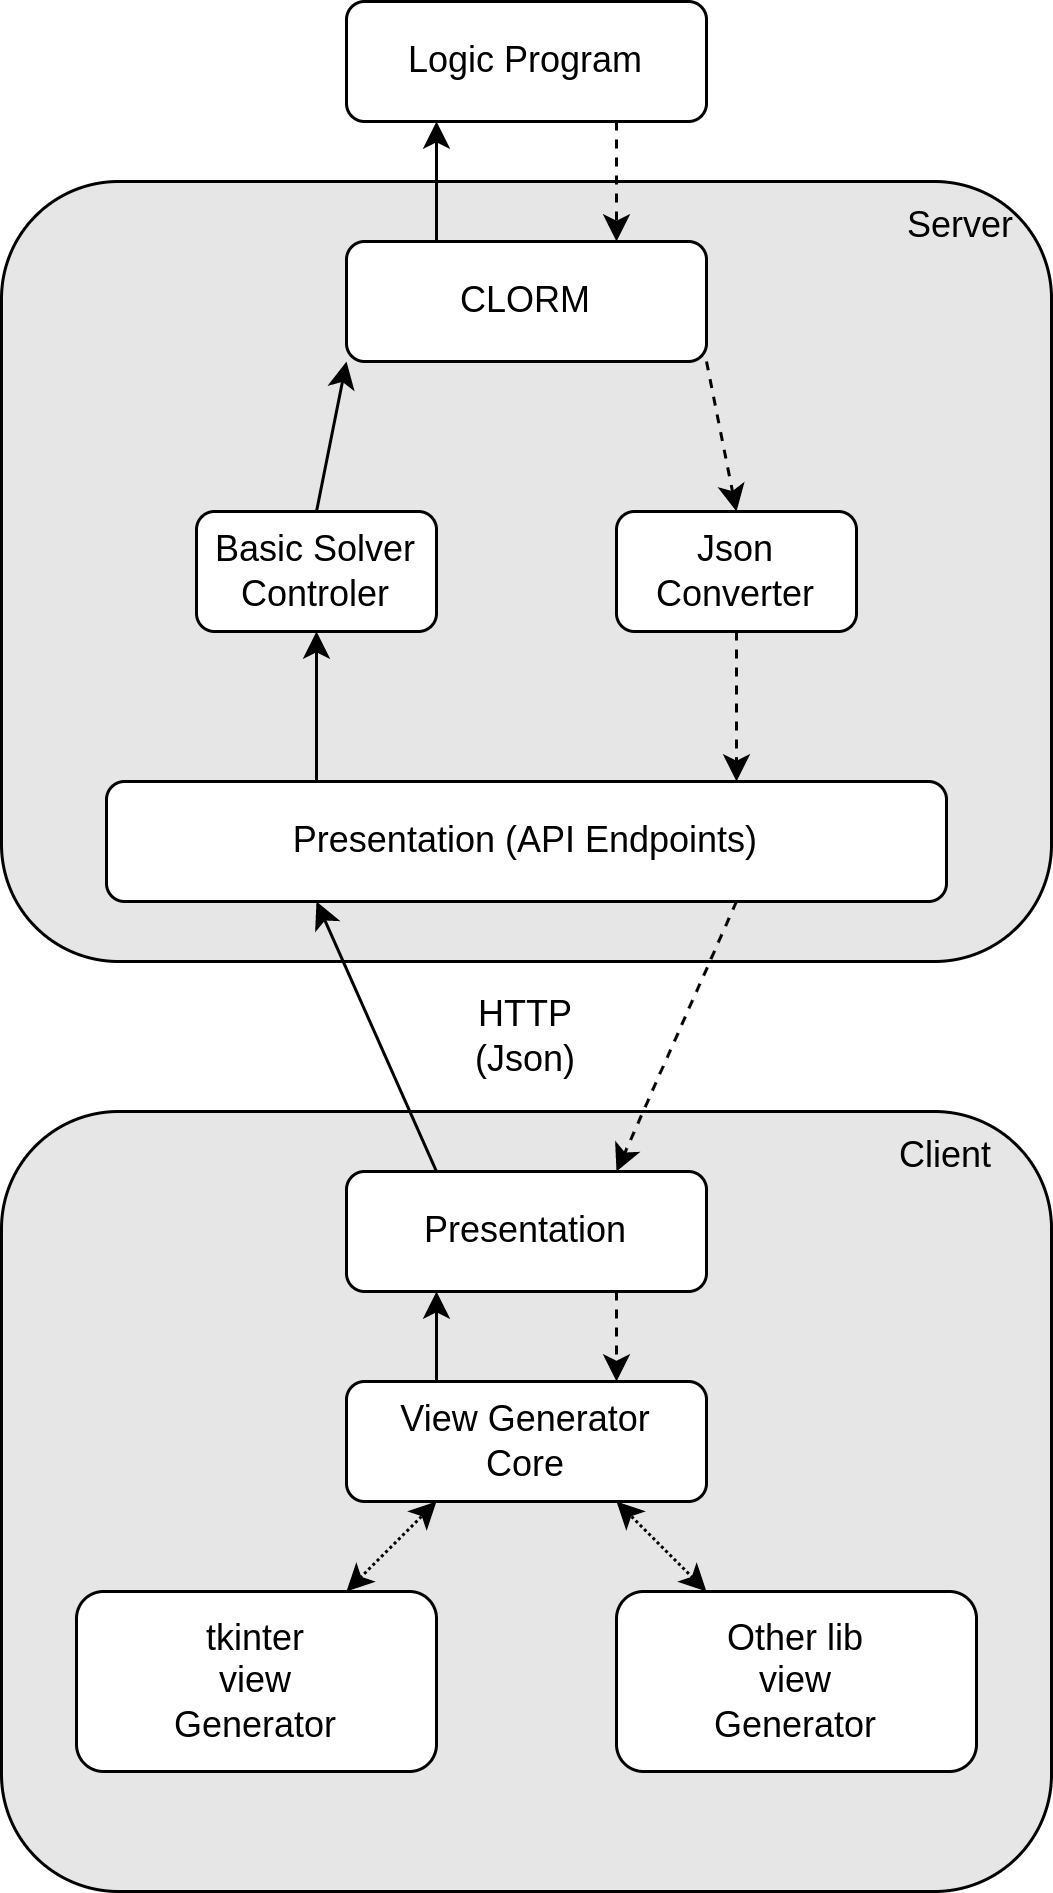
\includegraphics[width=0.3\textwidth]{imgs/client-server-v1.png}
    \caption{Cient-Server-v1 approach}
    \label{fig:client-server-v1}
    \end{center}
\end{figure}

\noindent The idea for the backend is now the following: The presentation layer consists of the API-endpoints, which just consists of two:

\begin{itemize}
    \item \textit{call} - POST: ''/'' - Solver function call.
    \item \textit{health} - GET: ''/health'' - For startup process, check if server is running.
\end{itemize}

\noindent When the \textit{call} endpoint receives a request, it looks at it and parses it (a request should look like a function call, so e.g. \textit{assume(sudoku(1,1,1))}). The function name must be a name of a function in the solver (e.g. \textit{assume}). The other payload may be used as one wishes.\\
Therefore the next step is to call the specified function in the solver, which processes the request and returns something (e.g. for the function \textit{solve()} this could be the Json representation of the whole GUI). For the conversion there should exist a Json-Converter which should be static in the sense, that every solver can use it easily.\\
As the previous line suggests, there will be many solvers. A user may specify a solver as one wants. The location of the solver (i.e. the module name in Python) can be specified as a command-line-argument (e.g. \textit{\$ clinguin --solver special-solver-1,special-solver-2 1.lp 2.lp 3.lp})\\[1em]
The first UML diagram depicts the use with the standard solver, the second one depicts a use with a special solver: 


\begin{figure}[ht]
    \begin{center}
    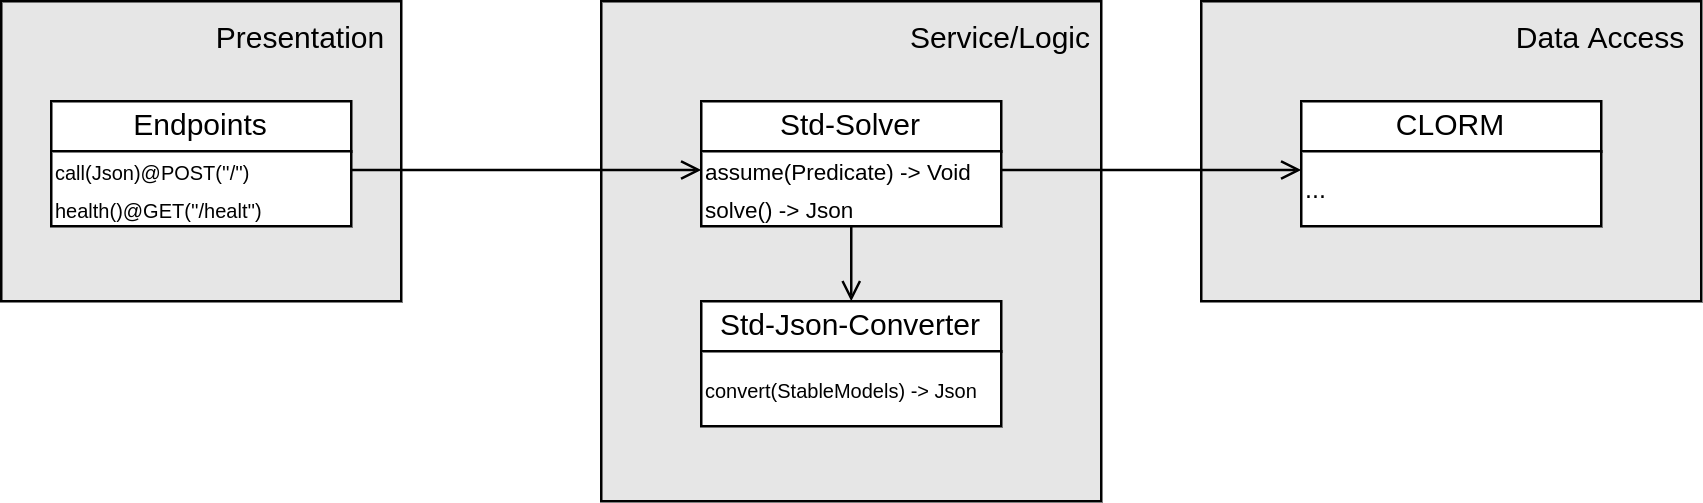
\includegraphics[width=0.6\textwidth]{imgs/uml-std-server.png}
    \caption{UML-Std.-Server}
    \label{fig:uml-std-server}
    \end{center}
\end{figure}

\begin{figure}[ht]
    \begin{center}
    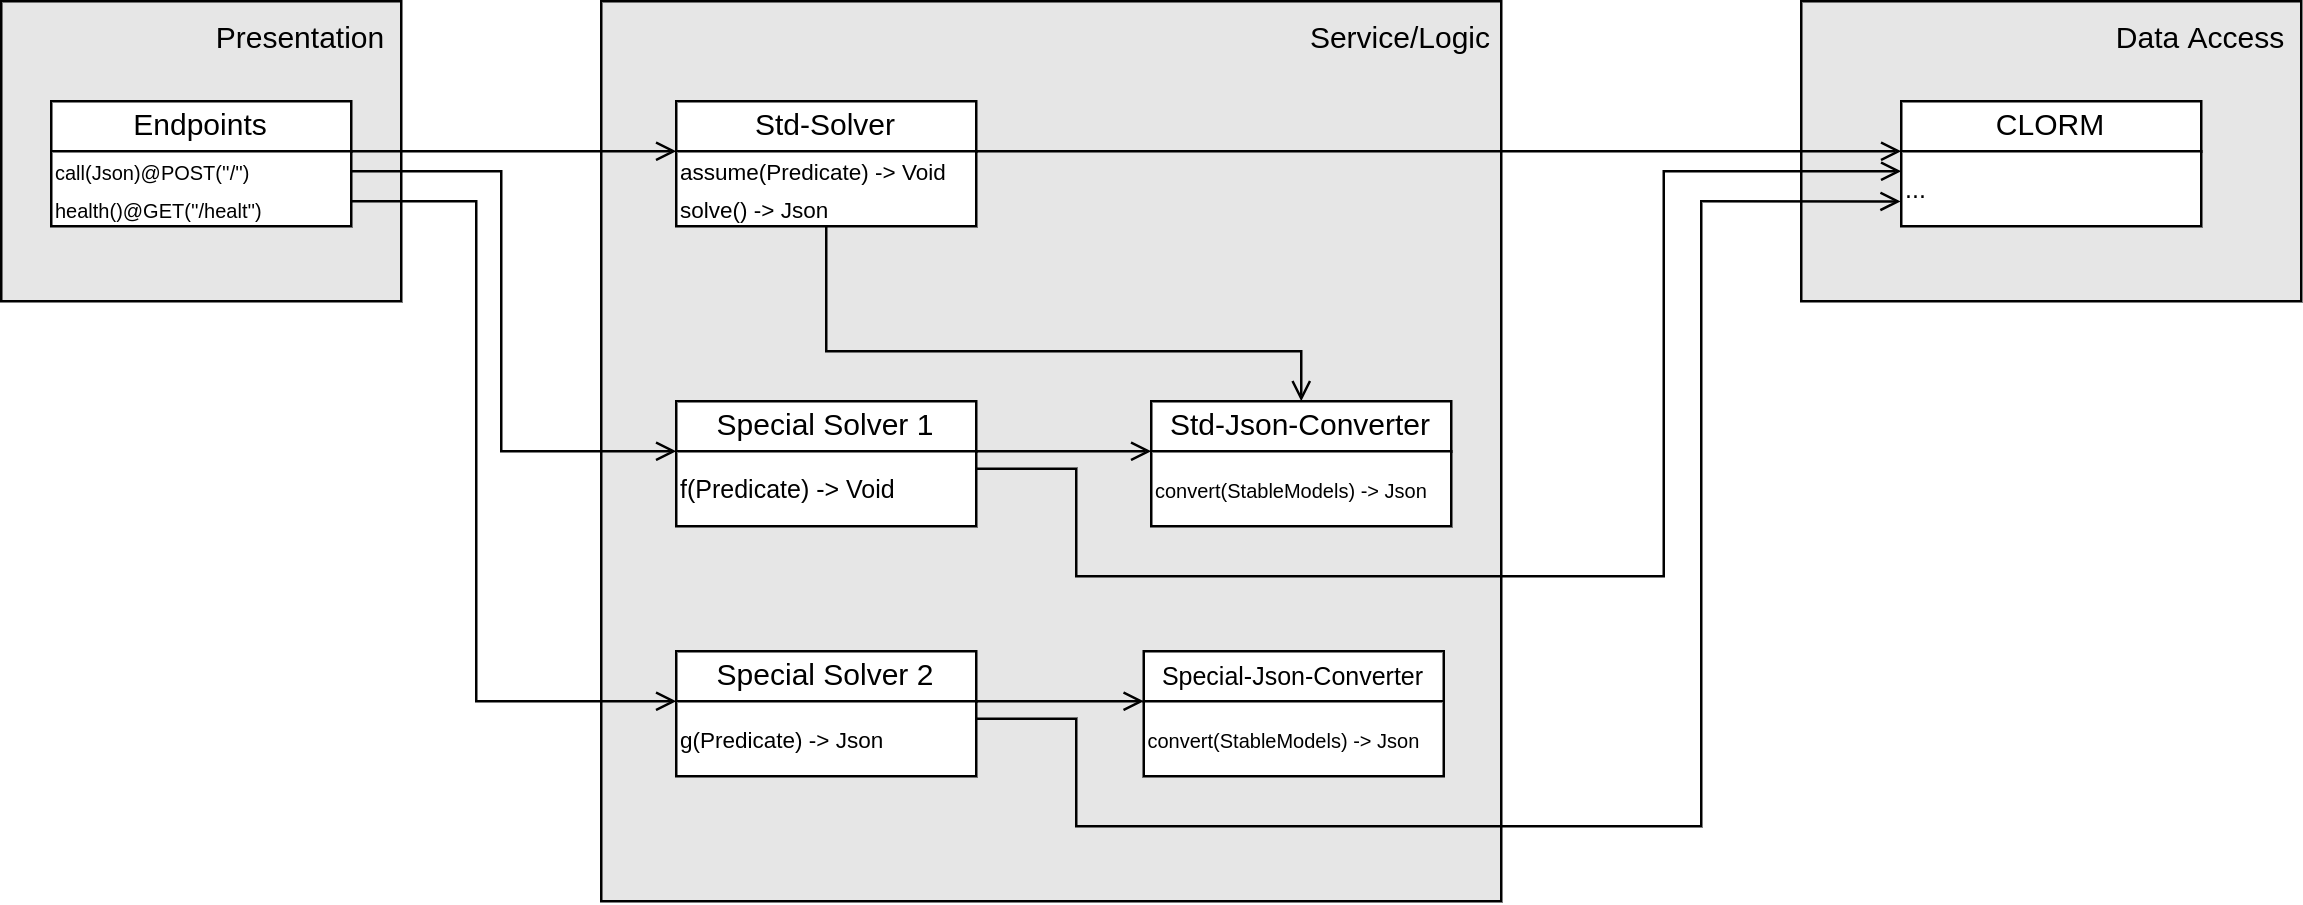
\includegraphics[width=0.6\textwidth]{imgs/uml-extended-server.png}
    \caption{UML-Extended-Server}
    \label{fig:uml-extended-server}
    \end{center}
\end{figure}


\noindent The client is also constructed in a way that should achieve, that one may switch from one python-gui framework to another. This is achieved, by splitting up the engine into a base engine (traverses the Json tree) and calling then the right method. This selection what to call is done by dependency injection. What engine to use can be specified by a command-line-argument. The UML diagram (Figure \ref{fig:uml-client}) depicts how this should play out. The \textit{interface-mock} is a class that should not be instantiated, as it only contains empty/not callable functions, which shall be implemented by the actual gui-implementations. It is termed \textit{interface-mock} as interfaces do not exists, implementation wise it could be implemented as an abstract class (which exists in python through the \textit{ABC} library).

\begin{figure}[ht]
    \begin{center}
    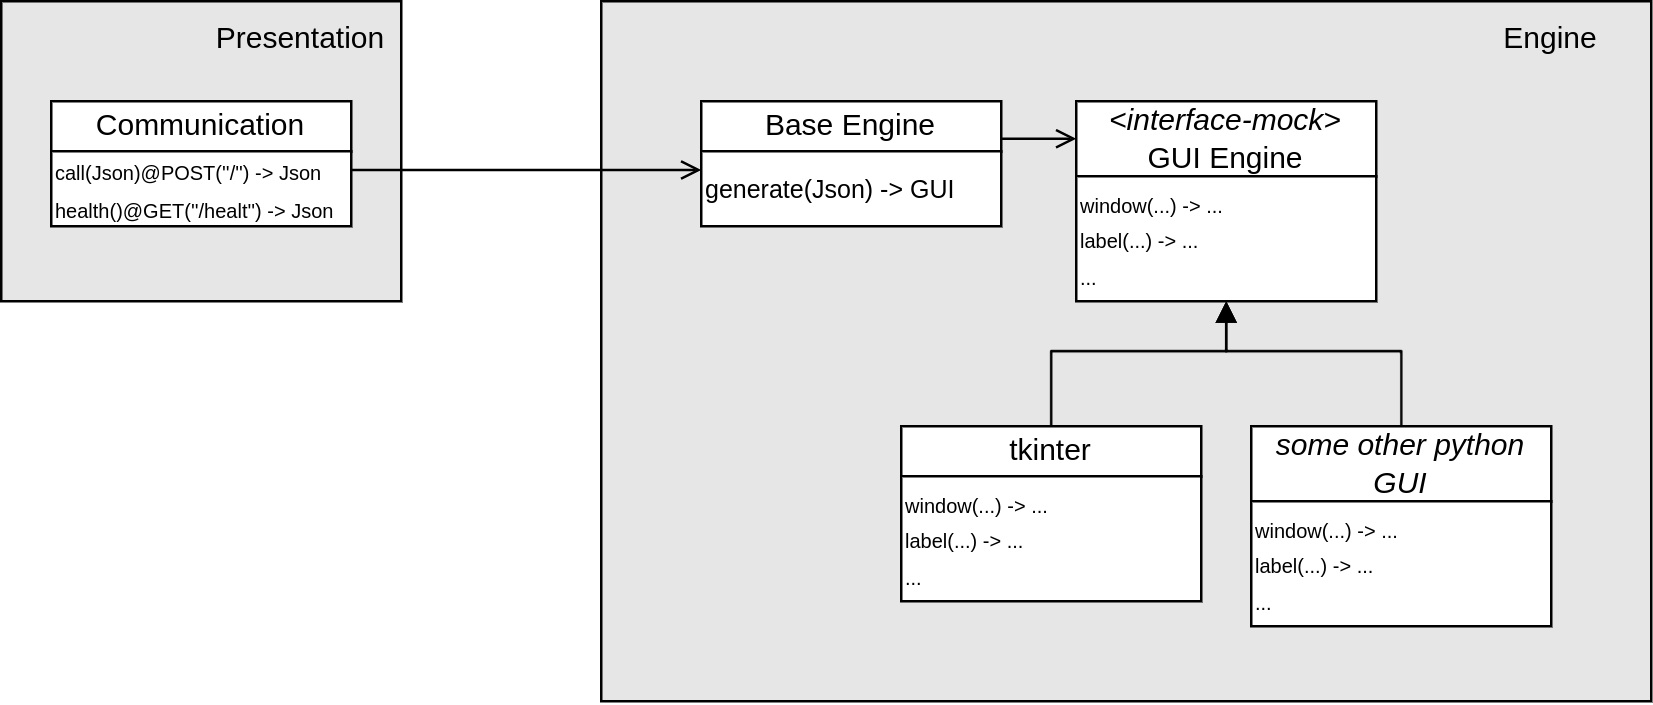
\includegraphics[width=0.6\textwidth]{imgs/uml-client.png}
    \caption{UML-Client}
    \label{fig:uml-client}
    \end{center}
\end{figure}


%%%%%%%%%%%%%%%%%%%%%%%%%%%%%%%%%%%%%%%%%
% Timestamp 12. - 18.07.2022
%%%%%%%%%%%%%%%%%%%%%%%%%%%%%%%%%%%%%%%%%
\newpage
\subsubsection{Version 2: An update}
\noindent Is based on \textit{Version 1} of the Client-Server-Architecture, a result from the meeting on the 11.07.2022 and is the first version, that shall be implemented as a prototype. The basic idea, that one implements the functionality with a Client-Server based architecture stays the same. The main difference between version \textit{1} and \textit{2} lies in the following:

\begin{itemize}
    \item Only one solver should be active at the time.
    \item For a first prototype only a very limited set of features shall be implemented (see syntax-definition of \textit{20220714\_alex\_syntax.lp}). In general the syntax shall be constructed in a more HTML way, therefore for example the possible values of a dropdown menu shall now be defined as seperate elements.
    \item For the prototype the Json-format the \textit{20220711\_alex\_json\_format.txt} will be used.
    \item For instrunctions how to execute the prototype see the \textit{/engine\_pt/README.md} Readme-file.
\end{itemize}

\noindent The following shows a more detailed view of the workings of the prototype. At first the general idea of this prototype is outlined, then sequence diagrams are shown and then a UML-Class diagram is shown:

\noindent \textbf{General Working:} 

\begin{figure}[ht]
    \begin{center}
    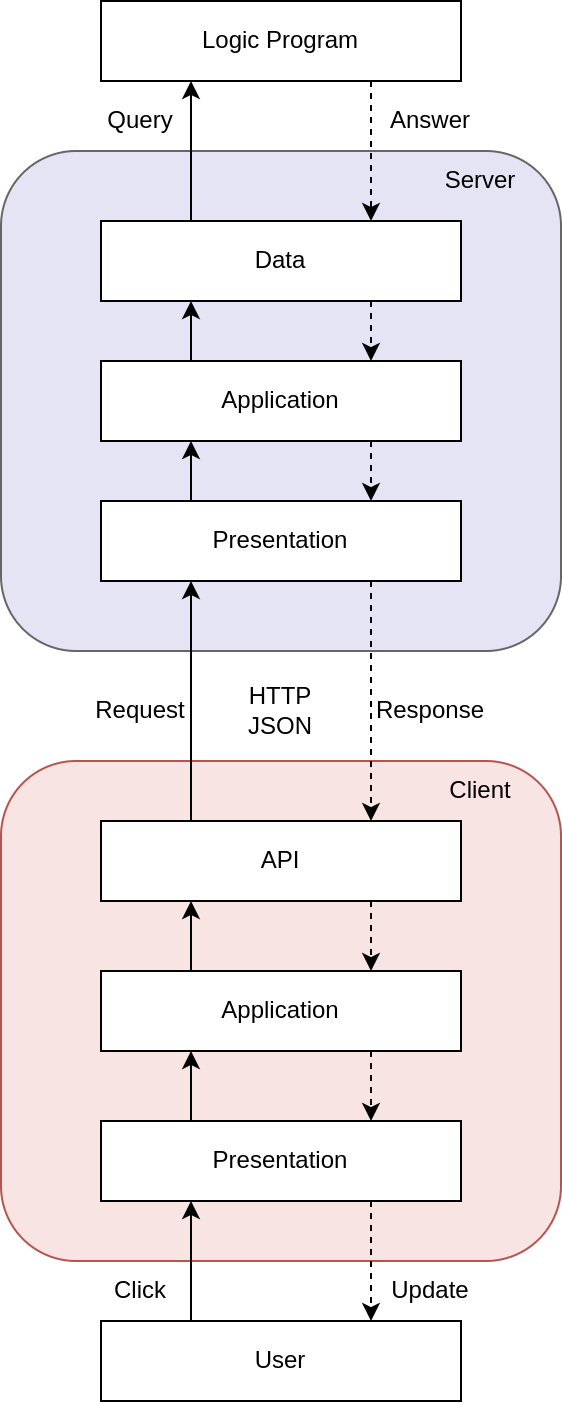
\includegraphics[width=0.3\textwidth]{imgs/pt-v2-server-client.png}
    \caption{Architectural Overview}
    \label{fig:pt-v2-server-client}
    \end{center}
\end{figure}

\newpage

\noindent \textbf{Sequence Diagrams}

\begin{figure}[ht]
    \begin{center}
    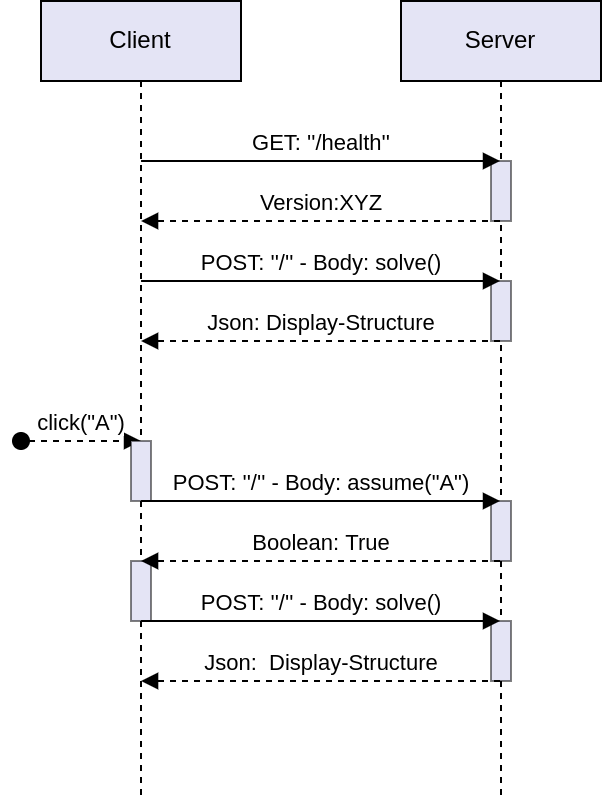
\includegraphics[width=0.3\textwidth]{imgs/pt-v2-sequence-normal.png}
    \caption{Sequence Diagram Normal}
    \label{fig:pt-v2-sequence-normal}
    \end{center}
\end{figure}


\begin{figure}[ht]
    \begin{center}
    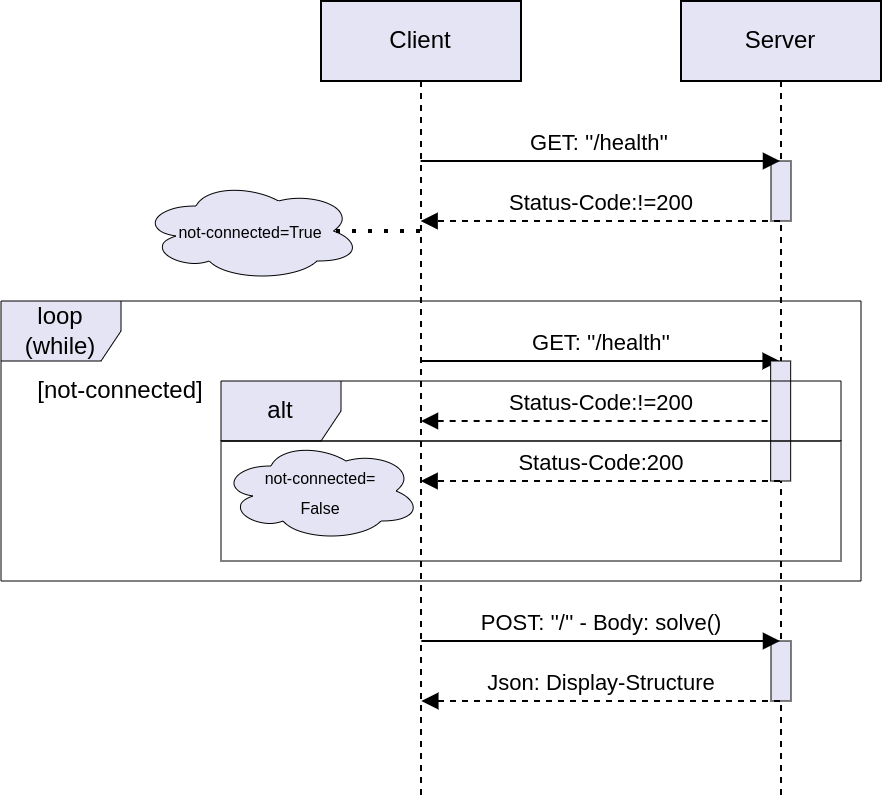
\includegraphics[width=0.3\textwidth]{imgs/pt-v2-sequence-failure.png}
    \caption{Sequence Diagram Failure}
    \label{fig:pt-v2-sequence-failure}
    \end{center}
\end{figure}

\newpage

\noindent \textbf{Class Diagram}

\begin{figure}[ht]
    \begin{center}
    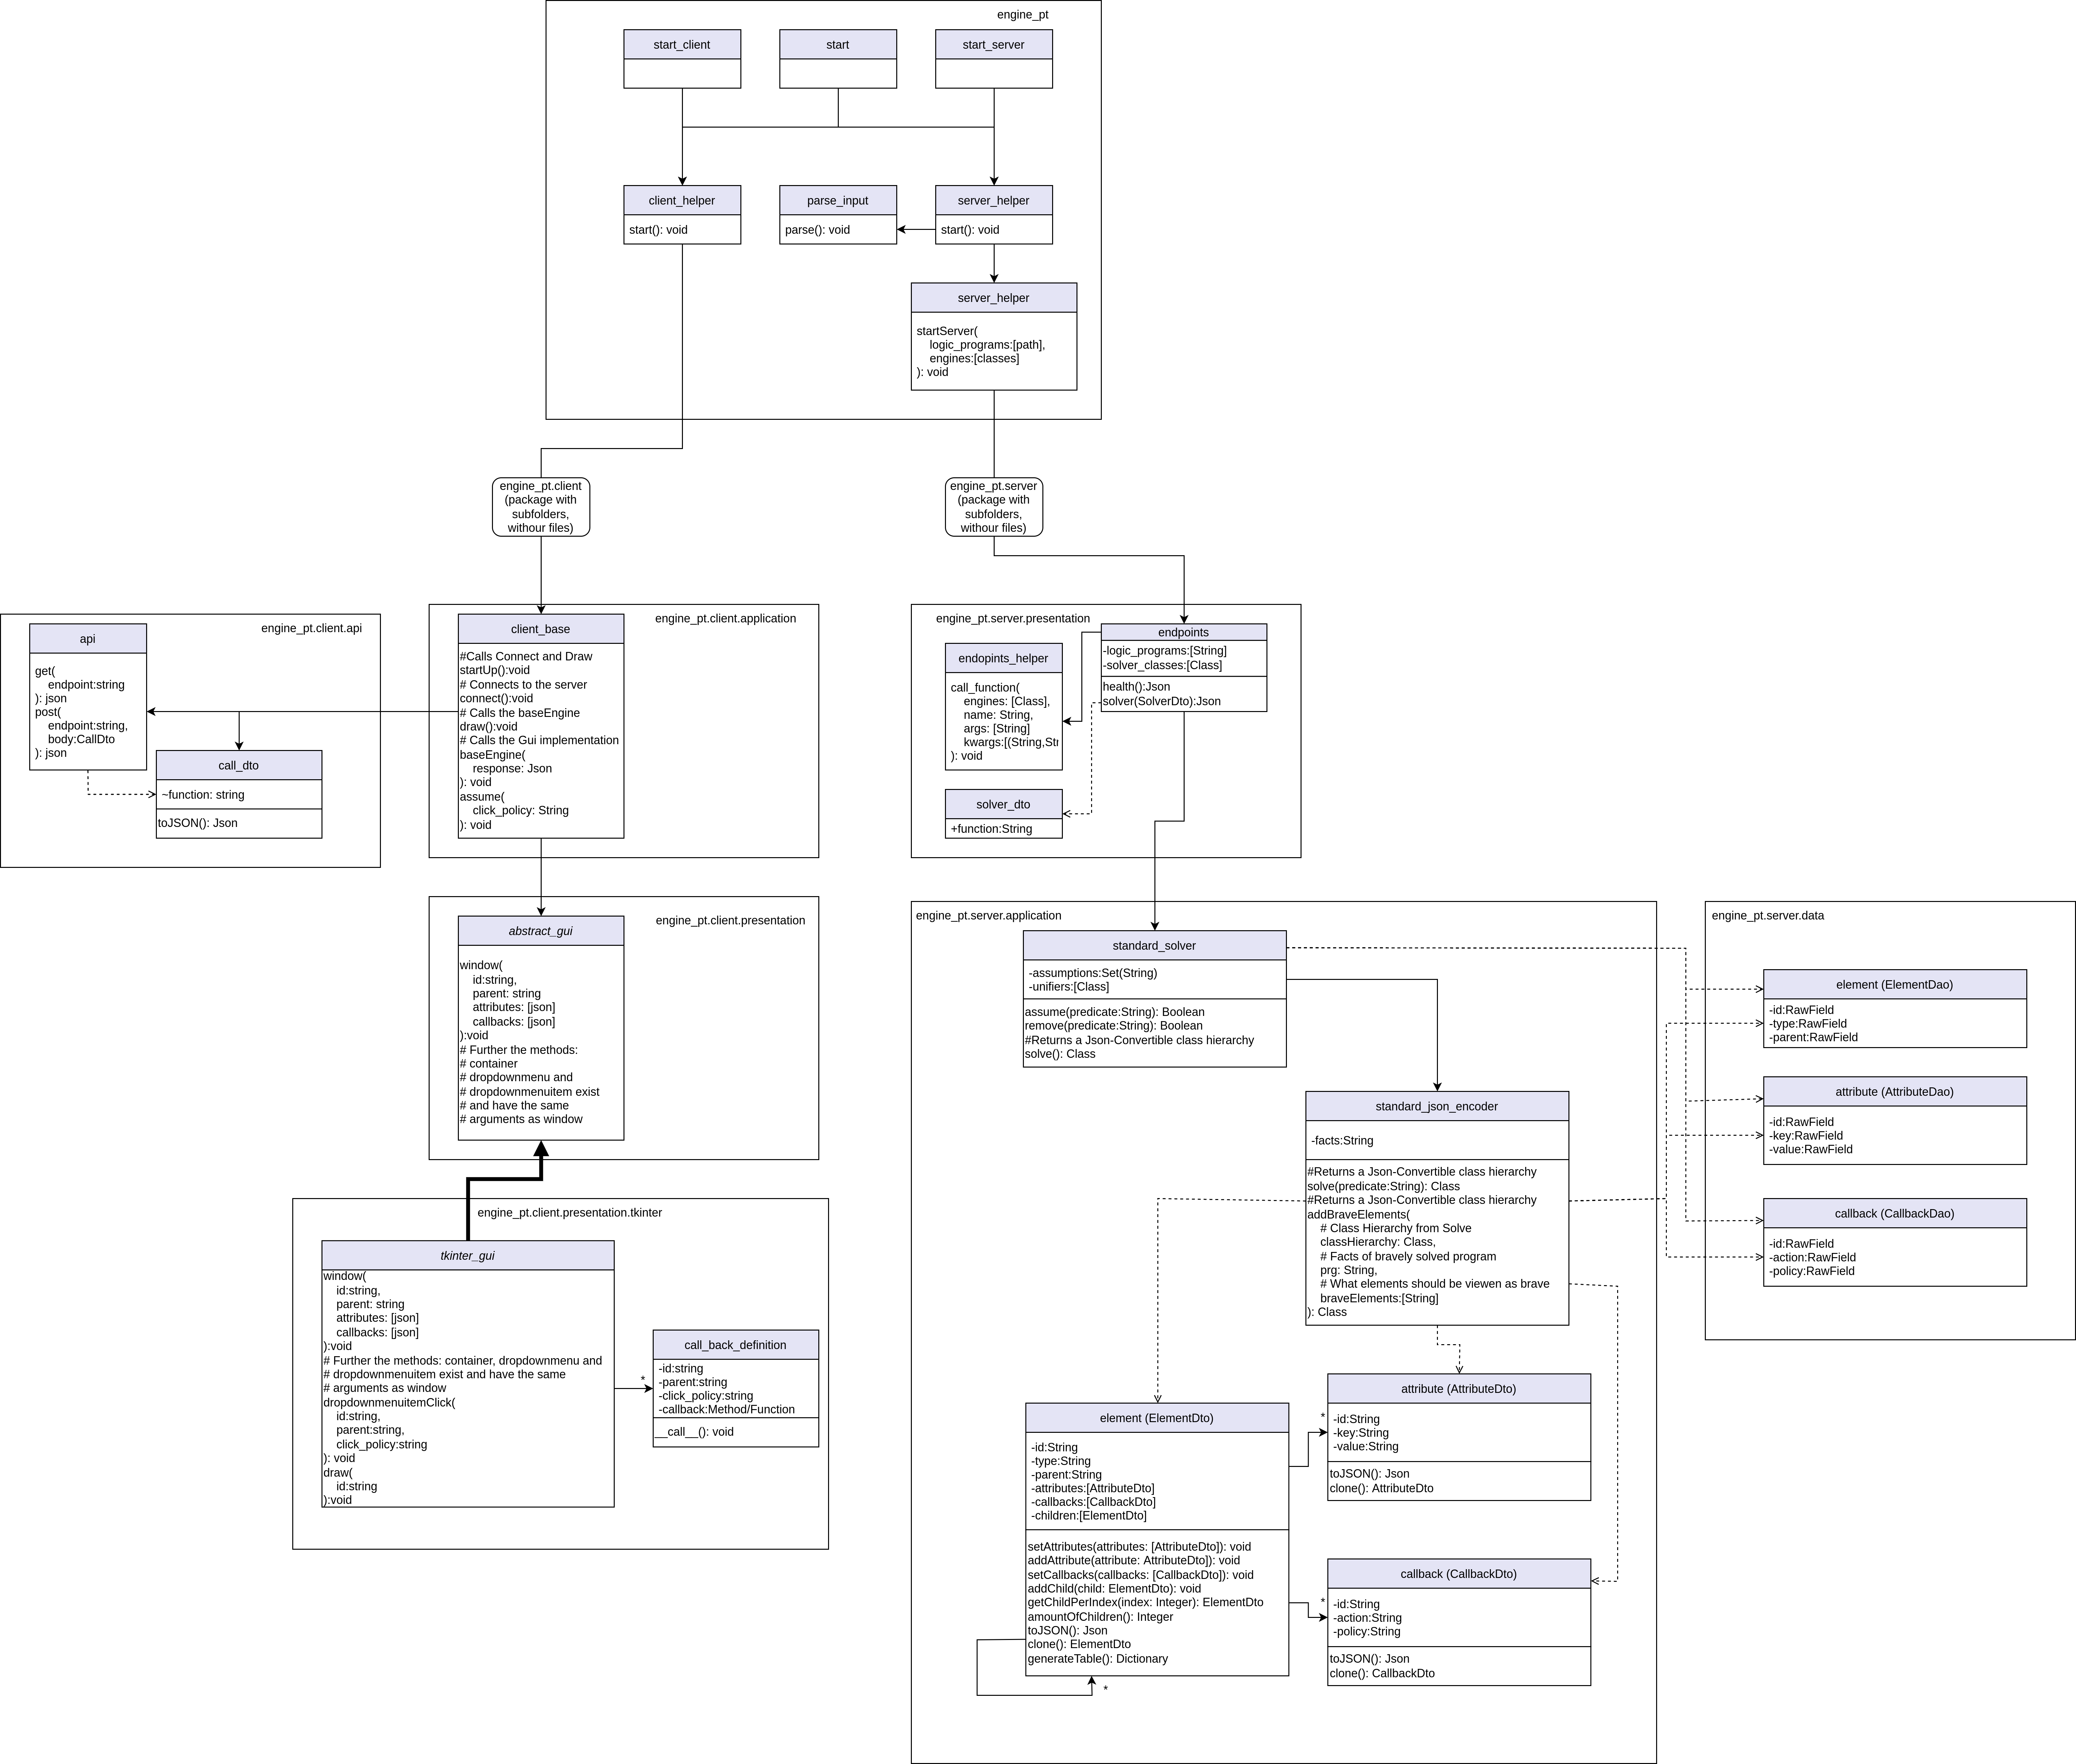
\includegraphics[width=0.9\textwidth]{imgs/pt-v2-class-diag.png}
    \caption{Class Diagram}
    \label{fig:pt-v2-class-diag}
    \end{center}
\end{figure}



























\end{document}












